\documentclass{article}
\usepackage{graphicx}
\usepackage{amsmath}
\usepackage{fancyhdr}
\usepackage[colorlinks=true, linkcolor=cyan, citecolor=cyan, urlcolor=green]{hyperref}
\pagestyle{fancy}
\lhead{Ali Abdollahi}
\rhead{Project 2}
\cfoot{Page \thepage}
\title{The Third Project\\\large Encoding \& Learning}
\begin{document}
	\maketitle
	\section{Encoding}
	Three encodings models were utilized in this project. Time to first spike, Poisson, and Positional coding. The 12 images were shown in the figure\ref{im}. All of the encoding functions, codes any image to a desired number of neurons and time. For down sampling the number of pixels, two methods were utilized. First, average and max pooling. And second, choosing a random sample of the pixels. 
	
	\begin{figure}[h]
		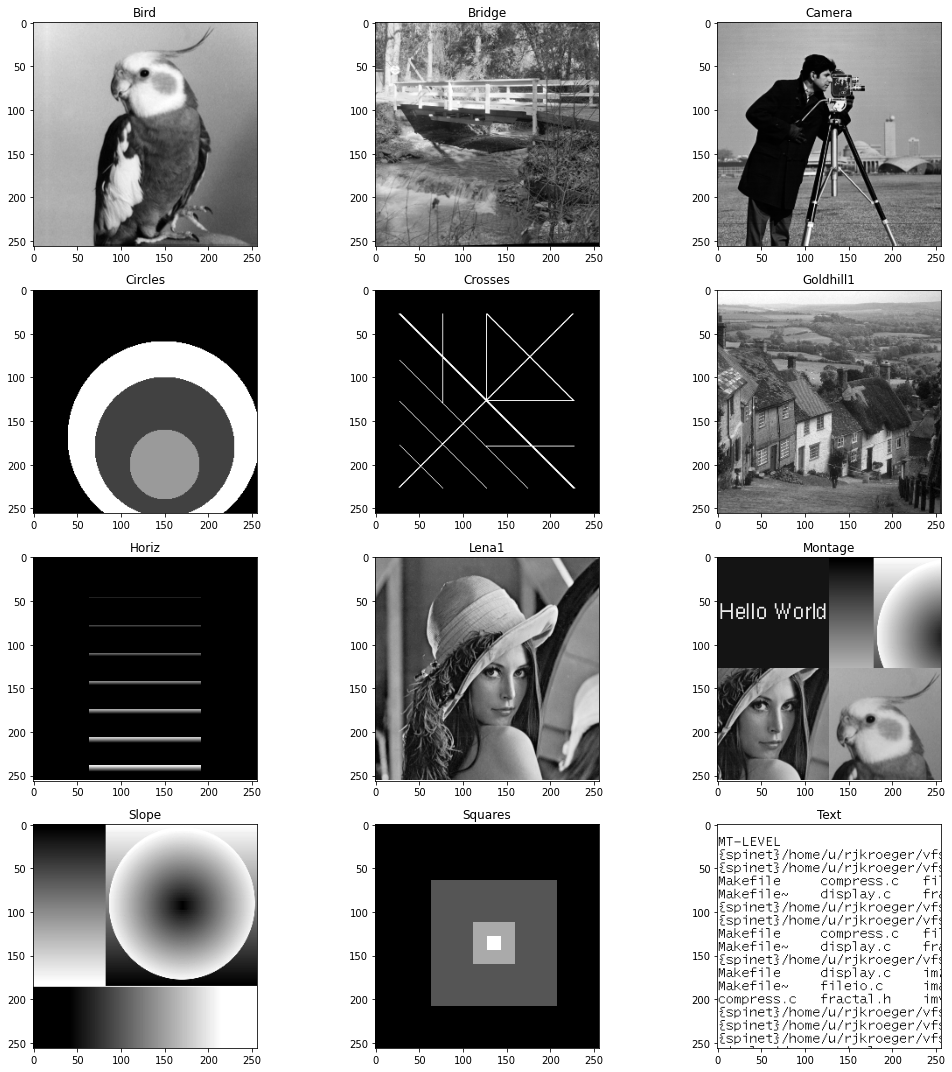
\includegraphics[width=1.2\textwidth]{images.png}
		\caption{The 12 images from this \href{https://links.uwaterloo.ca/Repository.html}{repository}, which used for encoding.}
		\label{im}
	\end{figure}
	\subsection{Time To First Spike}
	In the time to first spike method, only the first spike of each neuron matters. Thus, the coding is far sparser than the following encodings. These encodings are depicted in figure\ref{imttfs}.
	\begin{figure}[h]
		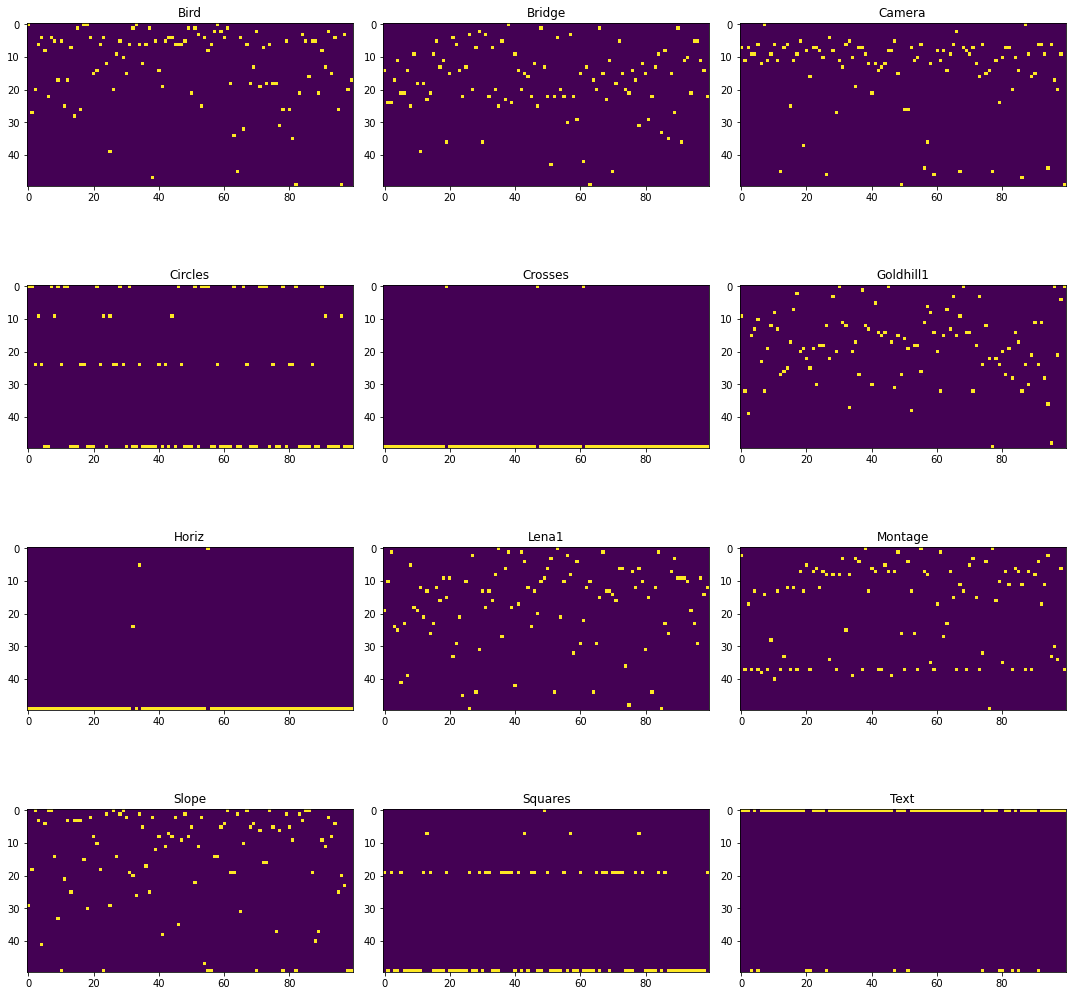
\includegraphics[width=1.2\textwidth]{images_ttfs.png}
		\caption{The TTFS encoding of the selected 12 images. The X-axis represents neurons and the Y-axis represents time}
		\label{imttfs}
	\end{figure}
	
	In the three of the images, crosses, text, and horiz, because most of the image is same and there is no complexity, the encodings are simple. For instance, in the crosses  and in the horiz, almost all of the neurons fires in the end, as most of the pixels are same. For circles and Squares, thanks to 4 spectrum of gray, there are 4 time steps where the corresponding neurons fire.
	\subsection{Poisson Coding}
	A random Poisson sample is generated for each value.
	
	\begin{figure}[h]
		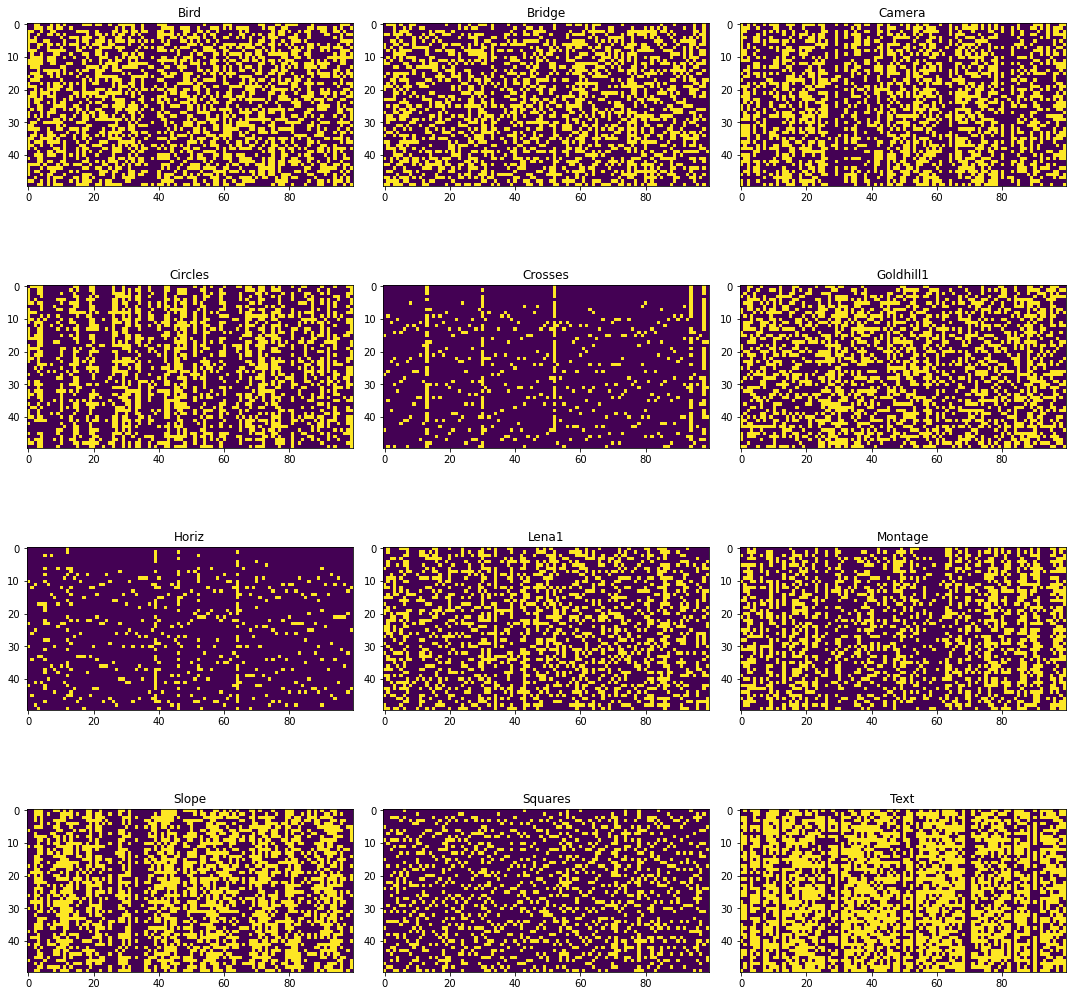
\includegraphics[width=1.2\textwidth]{images_poisson.png}
		\caption{The positional Coding of the images}
		\label{impois}
	\end{figure}
	
	As depicted in the plots, again for the crosses and the horiz, there is much less activity, because most of the pixels are 0. For text, that is the opposite case. For circles, we can observe that some neurons spikes much more frequent than other, which implies the different scale of grays.
	
	\subsection{Positional Values Coding}
	With this encoding, each pixel corresponds to a number of neurons. Each of those, denotes a different Gaussian plot. Their means are scattered in the range of pixels, typically 256 ($ [0, 1]$ if pixels were normalized), and the neurons fire with respect to the point which the desired value line intersects it. Thus, the closer the value to the mean, the earlier it fires (or if desired, the later it fires). 
	
	For efficiency, we did not compute all the neurons' probability density function (PDF). But rather the closest neuron is calculated, and the the nearest three from right and left were participated in this operation. Therefore, instead of calculating the PDF for $N$ normal distributions, only a small number (in our experiment 6) were selected.
	
	\begin{figure}[h]
		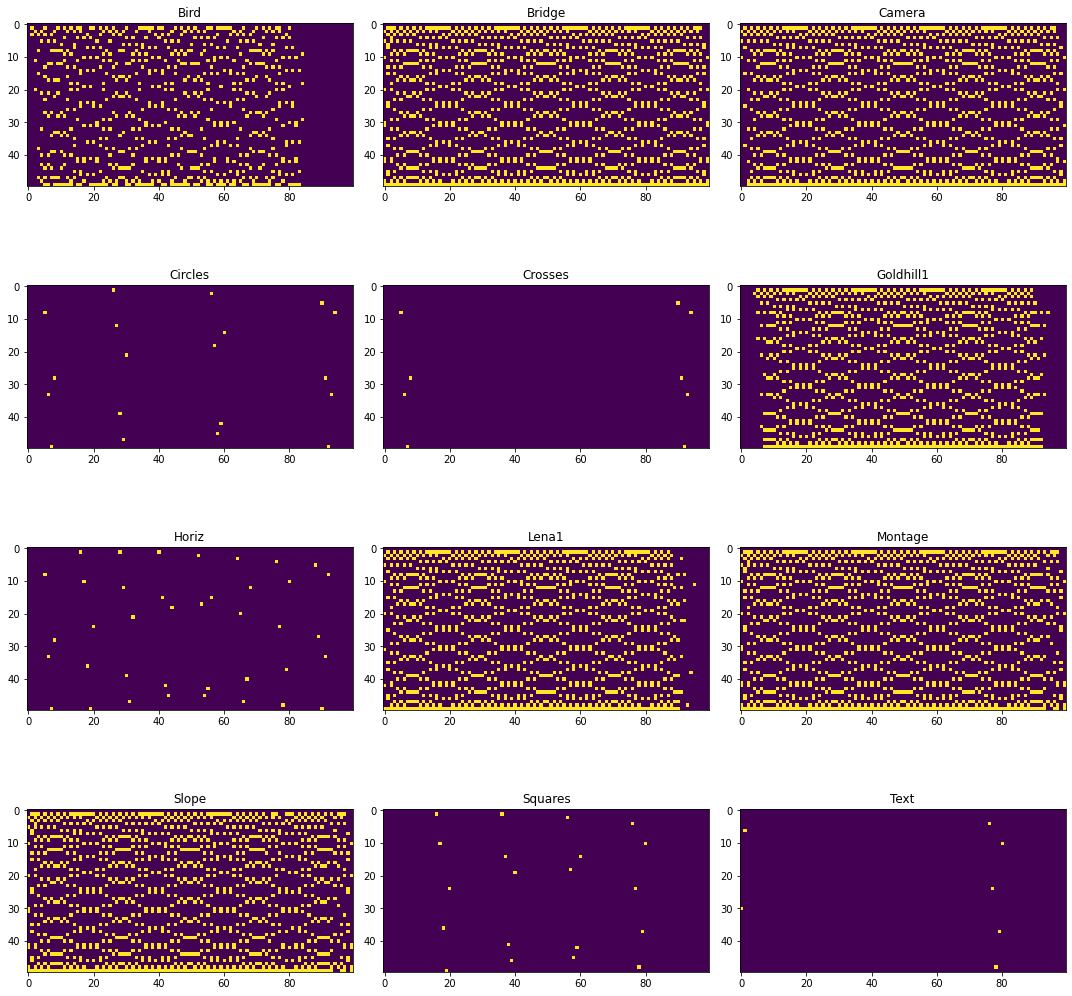
\includegraphics[width=1.2\textwidth]{images_pos.png}
		\caption{The positional Coding of the images}
		\label{impos}
	\end{figure}
	
	\section{STDP}
	\subsection{Input}
	The input of this \textbf{STDP} was an image per time. An image is selected randomly and the encoding calculated while adding an specified number of zeros to simulate a blink (or sleep). Then, those spikes are fed into the model. This process repeated for 55 iterations- The actual iterations number is 55 times the sum of encoding and sleep time ($15 + 5 = 20$) which equals $1100$ iterations.
	
	The two utilized patterns was the Poisson encoding \textit{`Lena`} and \textit{`Crosses`}, because their difference was substantial and learning to differentiate them is more achievable!
	
	\subsection{Weights}
	The weights are randomly initiated with a Gaussian distribution of $\mathcal{N}(50, 5)$. In the figure \ref{fig:wchange}, we can see how the weighs changed through these iterations. Every time some weights experiences some changes, the reverse was applied to the other weights, so that the sum of dendrites remain constant.
	
	The trend for the case which there is no intersection, shows that the first neurons which are responsible for the first image played a more important role, and this is true for both of the output neurons. The opposite is true for the other half of the input neurons, and they played an inhibitory role there.
	
	For trace, both the flat and non-flat methods have been implemented and tested. Although in the latter one, the last stimuli matter mostly, this is not completely true. Because biologically, the earlier the stimuli arrives, the more information it contains, as it can suggests us earlier hint about the future result. Therefore, for the following experiments, the flat-STDP has been utilized.
	\begin{figure}
		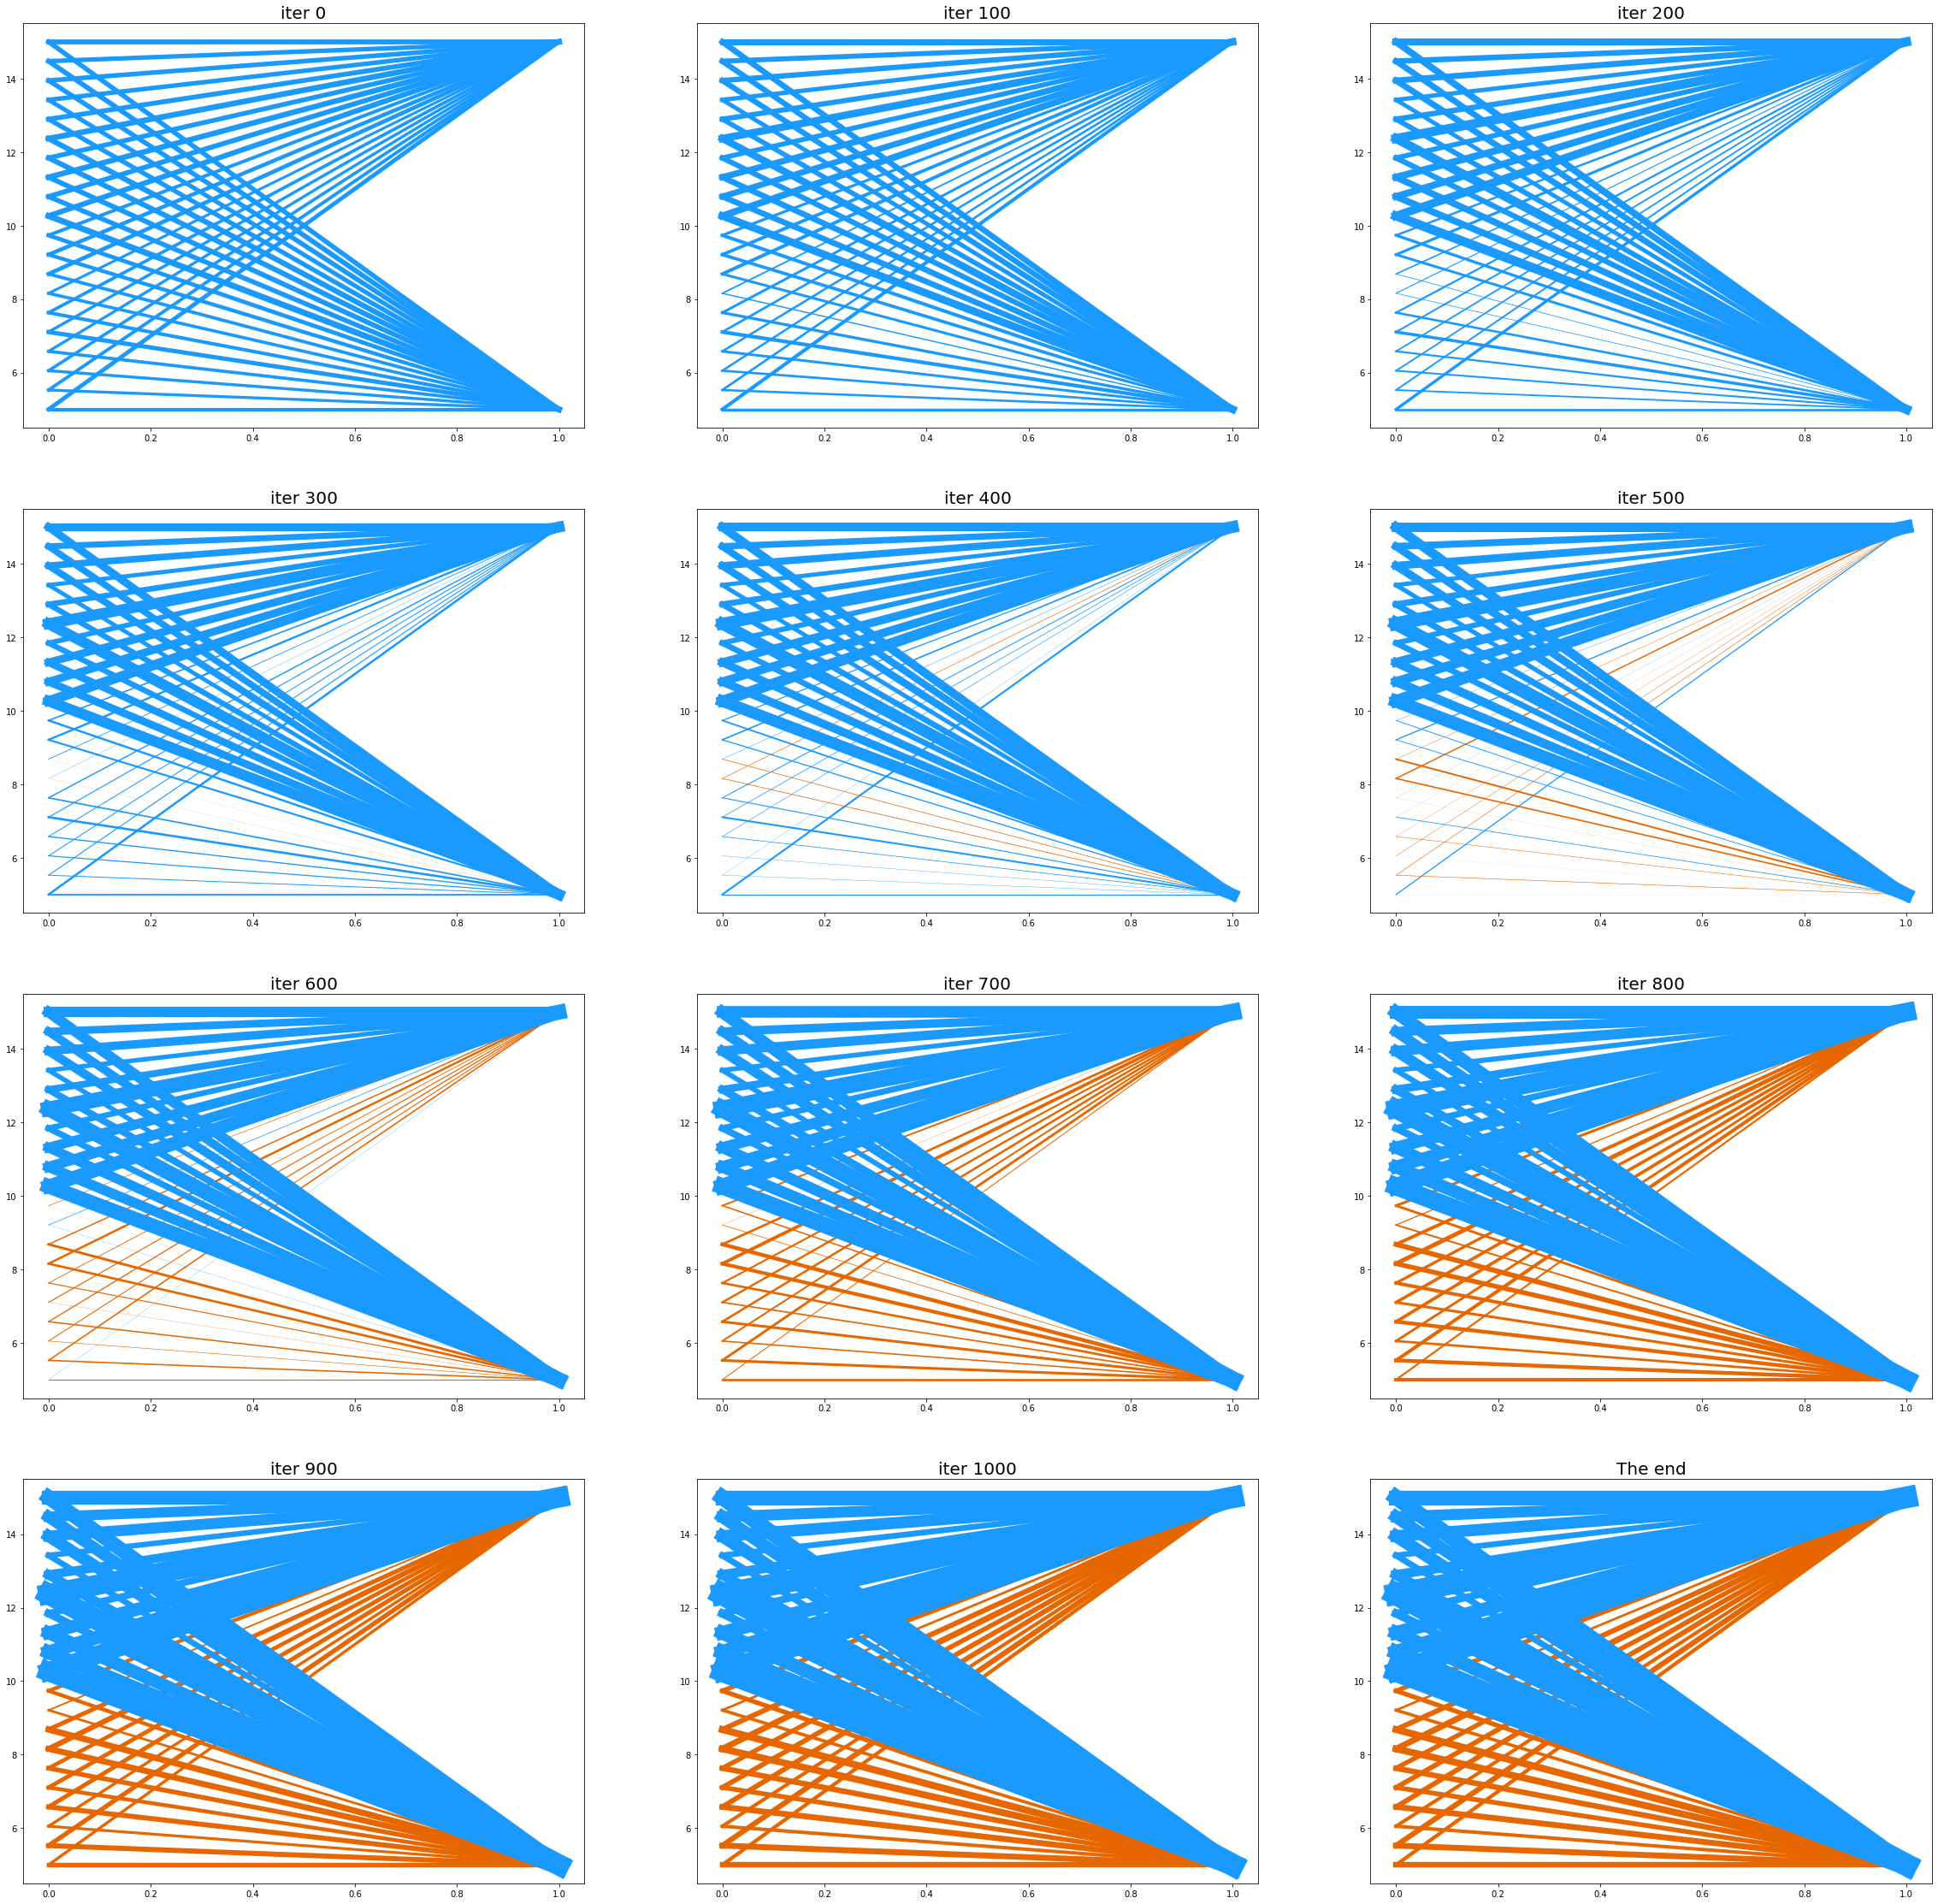
\includegraphics[width=\textwidth]{weight_change.png}
		\caption{The changes of synaptic weights through the time. The weights are captured every 100 iteration (or in another word every 5 image, as $T_{encoding}=15$ and $T_{sleep}=5$). The blue lines indicate positive, and the orange ones show negative weights. There was not intersected neurons. The first and second half of the input neurons shows \textit{`Crosses`} and \textit{`Lena`}, respectively.}
		\label{fig:wchange}
	\end{figure}
	
	In the figure \ref{fig:wchangerev}, the first neurons show the \textit{`Lena`}, and the next neurons shows the \textit{`Crosses`}. As we can observe, in this time the first neurons shows inhibitory behavior. This is a sign that the sparser pattern becomes the excitatory and vice versa.

	What can be the reason? The equation \ref{eq:dw} shows how the $dw$ is calculated. A possible explanation could be the following:
	
	\begin{equation}
		dw = trace_{pre} * spikes_{post} - trace_{post} * spikes_{pre}
		\label{eq:dw}
	\end{equation} 
	
	In general, the $trace$s are smaller (they are a fraction). Moreover, $pre$ is smaller than the $post$. Therefore, $trace_{post} * spikes_{pre}$ is smaller than $trace_{pre} * spikes_{post}$ for sparser pattern. Thus, the $dw$ becomes bigger and bigger.
	\begin{figure}
		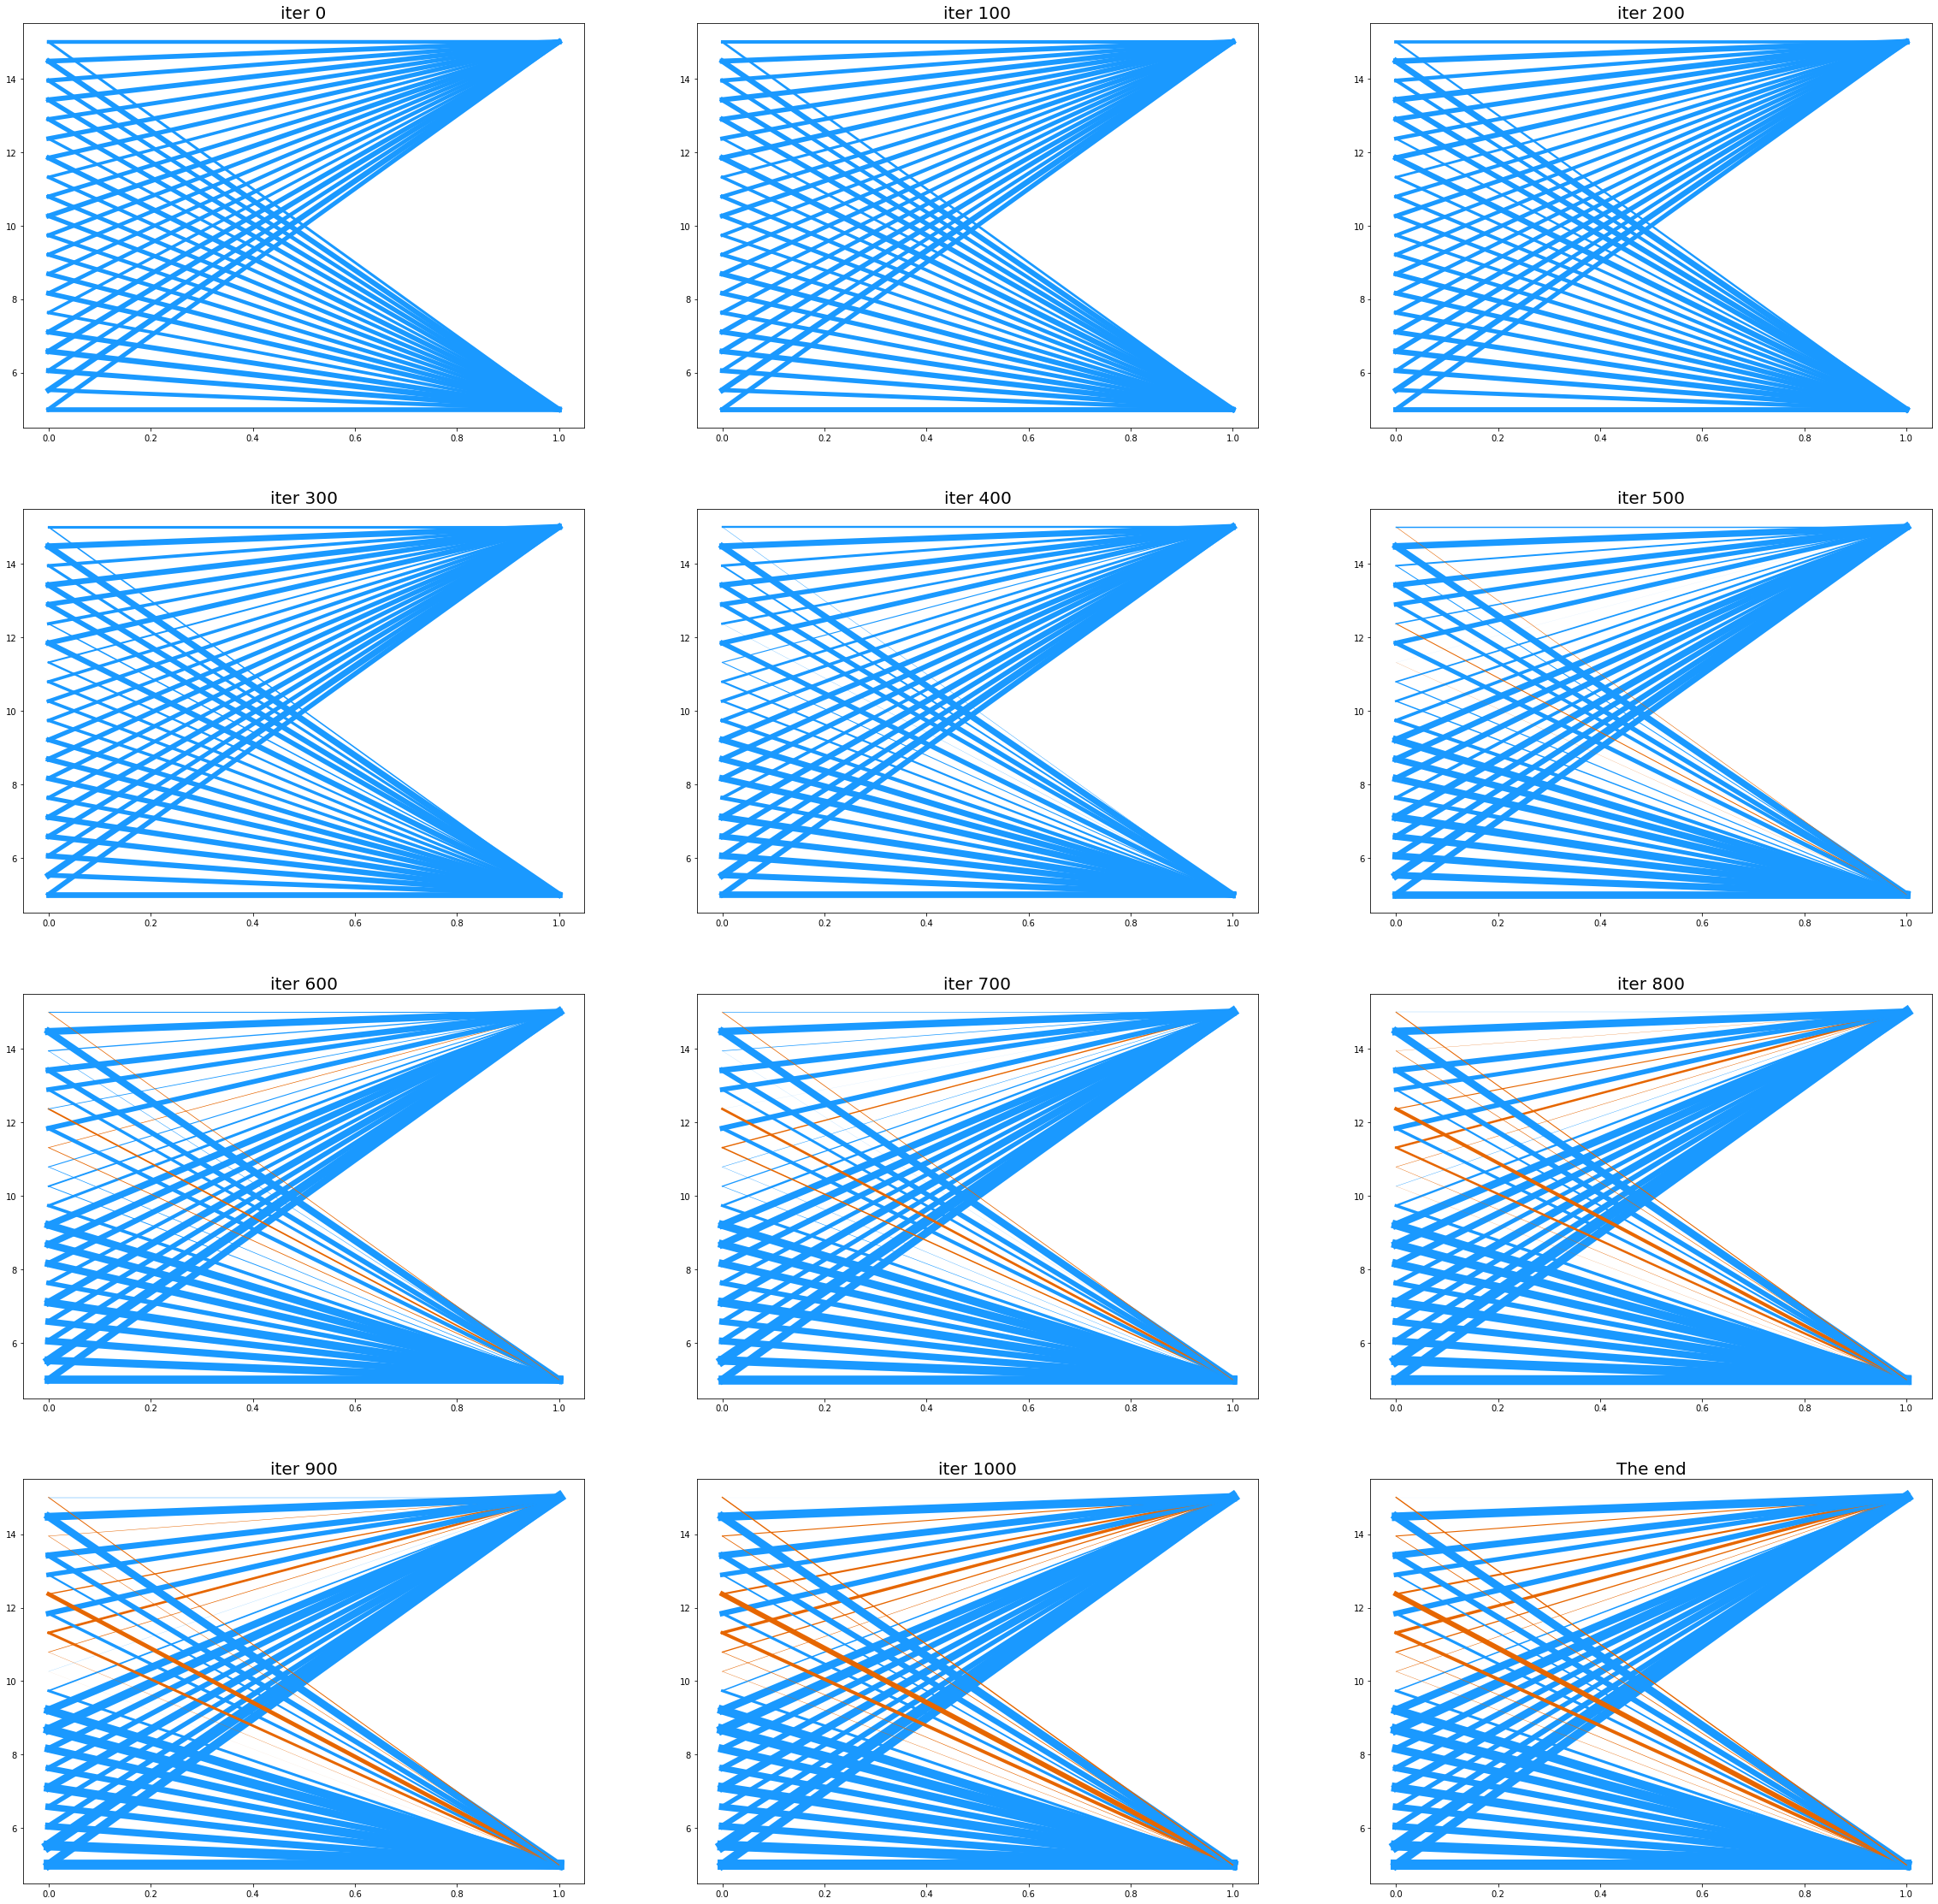
\includegraphics[width=\textwidth]{weight_change_reverse.png}
		\caption{Same as figure \ref{fig:wchange}, however the two images swapped so the first neurons shows the \textit{`Lena`} image, and the second ones are for \textit{`Crosses`}.}
		\label{fig:wchangerev}
	\end{figure}
	\subsubsection{Weights Similarity}
	The dendrites weights to each of the output neurons have been shown in table \ref{table:w}. The cosine similarity of these two arrays calculated and it is $\simeq 0.99767$. This shows that the input to both neurons are almost identical, and no pattern has been learned, although the patterns were vary a lot!
	\begin{table}
		\centering
		\begin{tabular}{|c|c|c|}
			\hline
			N1 & N2 & diff \\
			\hline
			81.98 & 78.05 & 3.93\\
			159.27 & 165.71 & -6.44\\
			161.36 & 145.38 & 15.98\\
			106.07 & 100.38 & 5.69\\
			147.0 & 145.49 & 1.51\\
			125.79 & 123.39 & 2.4\\
			168.63 & 156.89 & 11.74\\
			165.68 & 170.18 & -4.5\\
			142.01 & 139.32 & 2.69\\
			134.06 & 139.33 & -5.27\\
			-49.38 & -41.08 & -8.3\\
			53.54 & 43.54 & 10.0\\
			0.11 & -0.15 & 0.26\\
			-54.18 & -40.92 & -13.26\\
			-40.15 & -38.43 & -1.72\\
			-49.76 & -38.06 & -11.7\\
			-56.12 & -49.64 & -6.47\\
			-116.24 & -118.27 & 2.02\\
			-50.61 & -44.41 & -6.2\\
			-52.57 & -40.49 & -12.08\\
			\hline
		\end{tabular}
		\caption{The dendrites weights. Left column shows the input connections to the first, and the middle column demonstrates the input weights to the second output neurons. The cosine similarity is around 0.998\%.}
		\label{table:w}
	\end{table}
	\subsection{Test}
	The last part is to test the model with the both images. Figure \ref{fig:test1} demonstrates the results. Interestingly, both of the neurons have learned the first image, and none of them can recognize the second one. As noted earlier, the first image was \textit{`Lena`}, the denser pattern.
	
	This is because one of them has excitatory connections to both of the neurons, and the other one has all inhibitory effects. This leads us to the observed phenomena, where only one of the images can be recognized by both of the output neurons.
	\begin{figure}[h]
		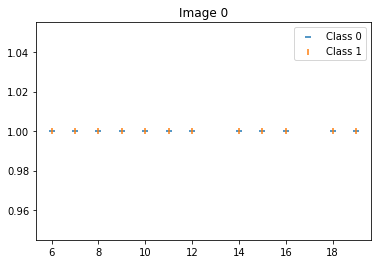
\includegraphics[width=0.5\textwidth]{test11.png}
		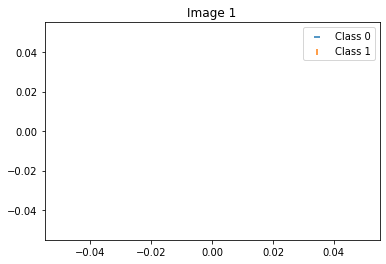
\includegraphics[width=0.5\textwidth]{test12.png}
		\caption{Spikes of the two neurons after training, when each of the images fed into the model. The blue horizontal and the orange vertical lines shows the first and second output neurons, respectively. Image 0 is \textit{`Lena`} and Image 1 is \textit{`Crosses`}.}
		\label{fig:test1}
		
	\end{figure}
	\subsection{More Intersection}
	In the previous cases, there was no intersection between the neurons that represents each image. Here, we want to explore two cases: first, 0.5 common neurons, and second, all the neurons are shared for both.
	
	In the figure \ref{fig:w50}, the first 10 neurons are in common for both patterns. the next 5 are for the first image, and the next 5 are for the second. In this case, the shared neurons played the inhibitory role. 
	\begin{figure}
		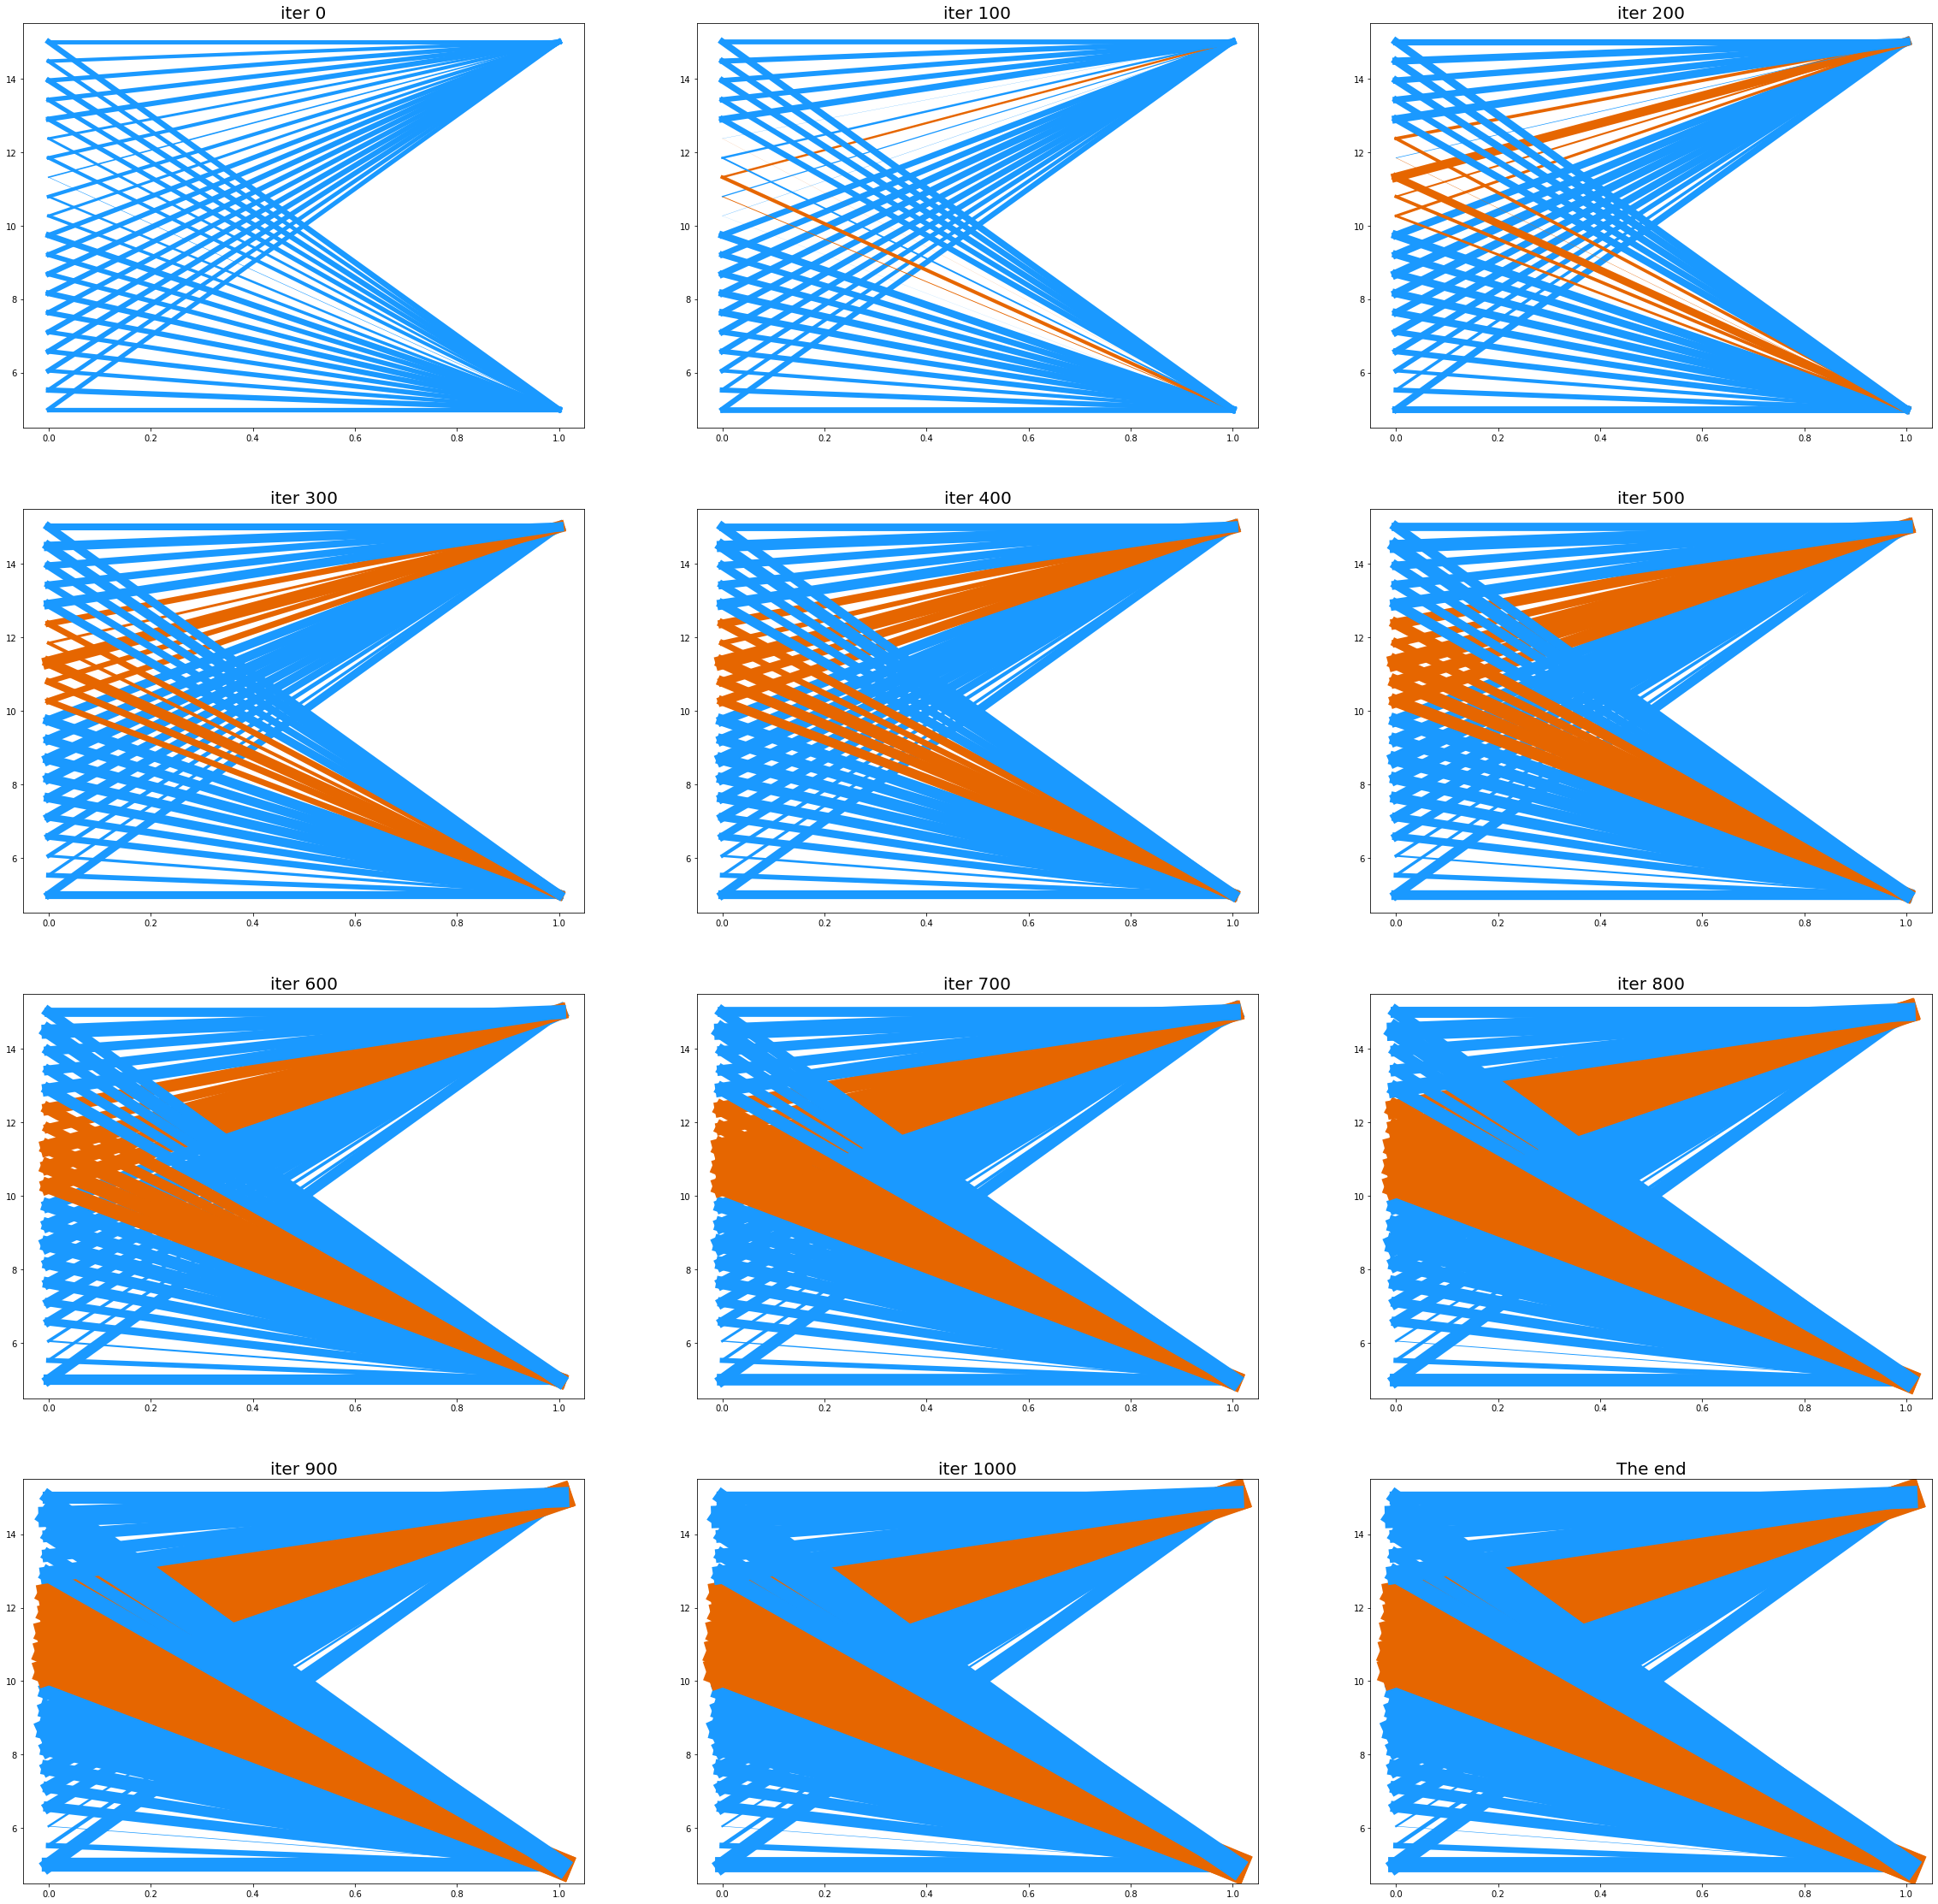
\includegraphics[width=\textwidth]{weight_change50.png}
		\caption{The weight change when there is a 50\%(first 10 neurons) intersection}
		\label{fig:w50}
	\end{figure}
	
	Like the previous case, the neurons which are devoted to the sparser pattern have inhibitory effect.
	
	\begin{figure}
		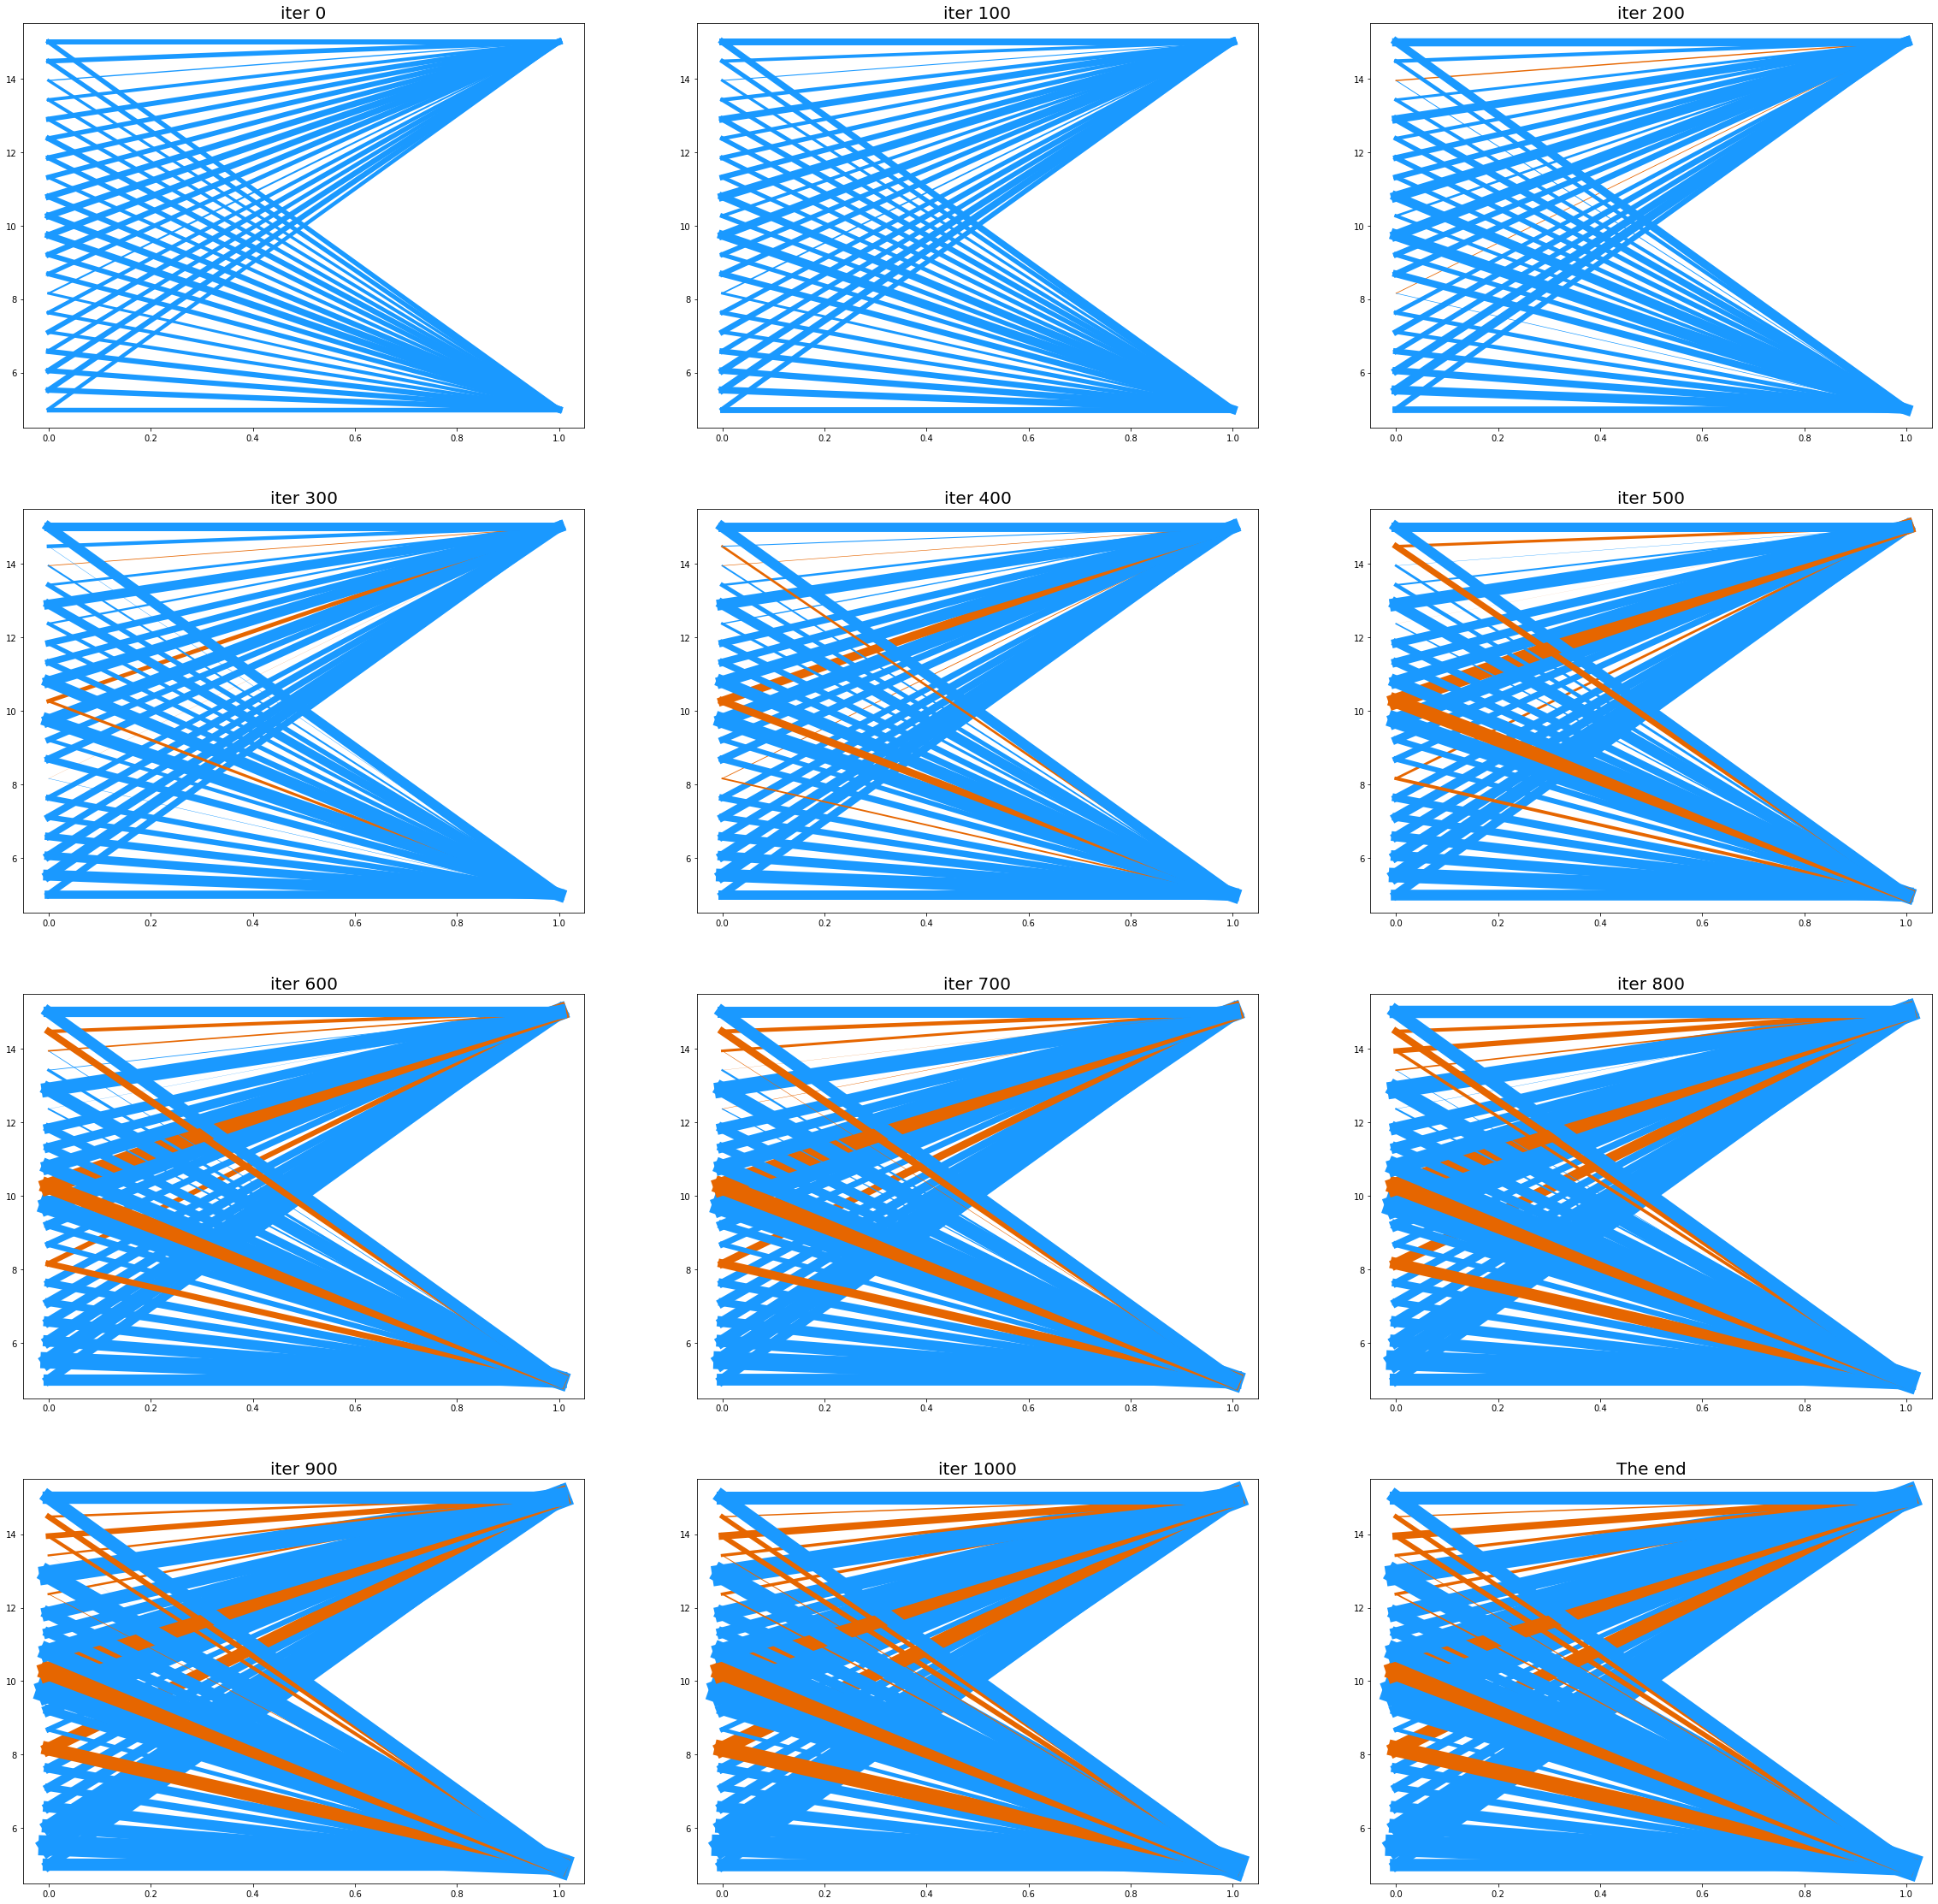
\includegraphics[width=\textwidth]{weight_change100.png}
		\caption{The weight change when all the neurons are in common}
		\label{fig:w100}
	\end{figure}
	
	Figure \ref{fig:w100} is when all the neurons are representing both of the images. 6 out of the 20 neurons play an inhibitory role, but this time it cannot be due to the input patterns. Moreover, with different executions, different neurons have negative weights.
	
	The cosine similarity in these both cases, remains the same (around 99\%). This shows that in general, STDP, due to its unsupervised nature, could not learn very good, even these two simply-differentiating patterns.
	
	\section{R-STDP}
	When adding reward, we have the ability to control the model, and we can reach to our expectations. Whenever any spikes occur during training, we compare it to the observing image at that time. If a neuron should (shouldn't) fire but it didn't (did), then we increase (decrease) the weights accordingly. This lets us to identify the pixels which can discriminate the two images.
	
	\subsection{Weights}
	Although in the STDP method, almost always the similarity between the input of the two neurons was more than 99\%, in the R-STDP learning model, this number vary a lot. Different executions leads the similarity in the range of 38\% to 80\%!
	
	Lots of factors are responsible for this diversity. Some of them are:
	\begin{itemize}
		\item[$\bullet$] The initial weights
		\item[$\bullet$] The encoding of the two images. How similar the two patterns are?
		\item[$\bullet$] The arrangement of inputs during learning.
	\end{itemize}
	They can be alleviated by data augmentation (fed different encoding of the images into the model).
	\begin{figure}[h]
		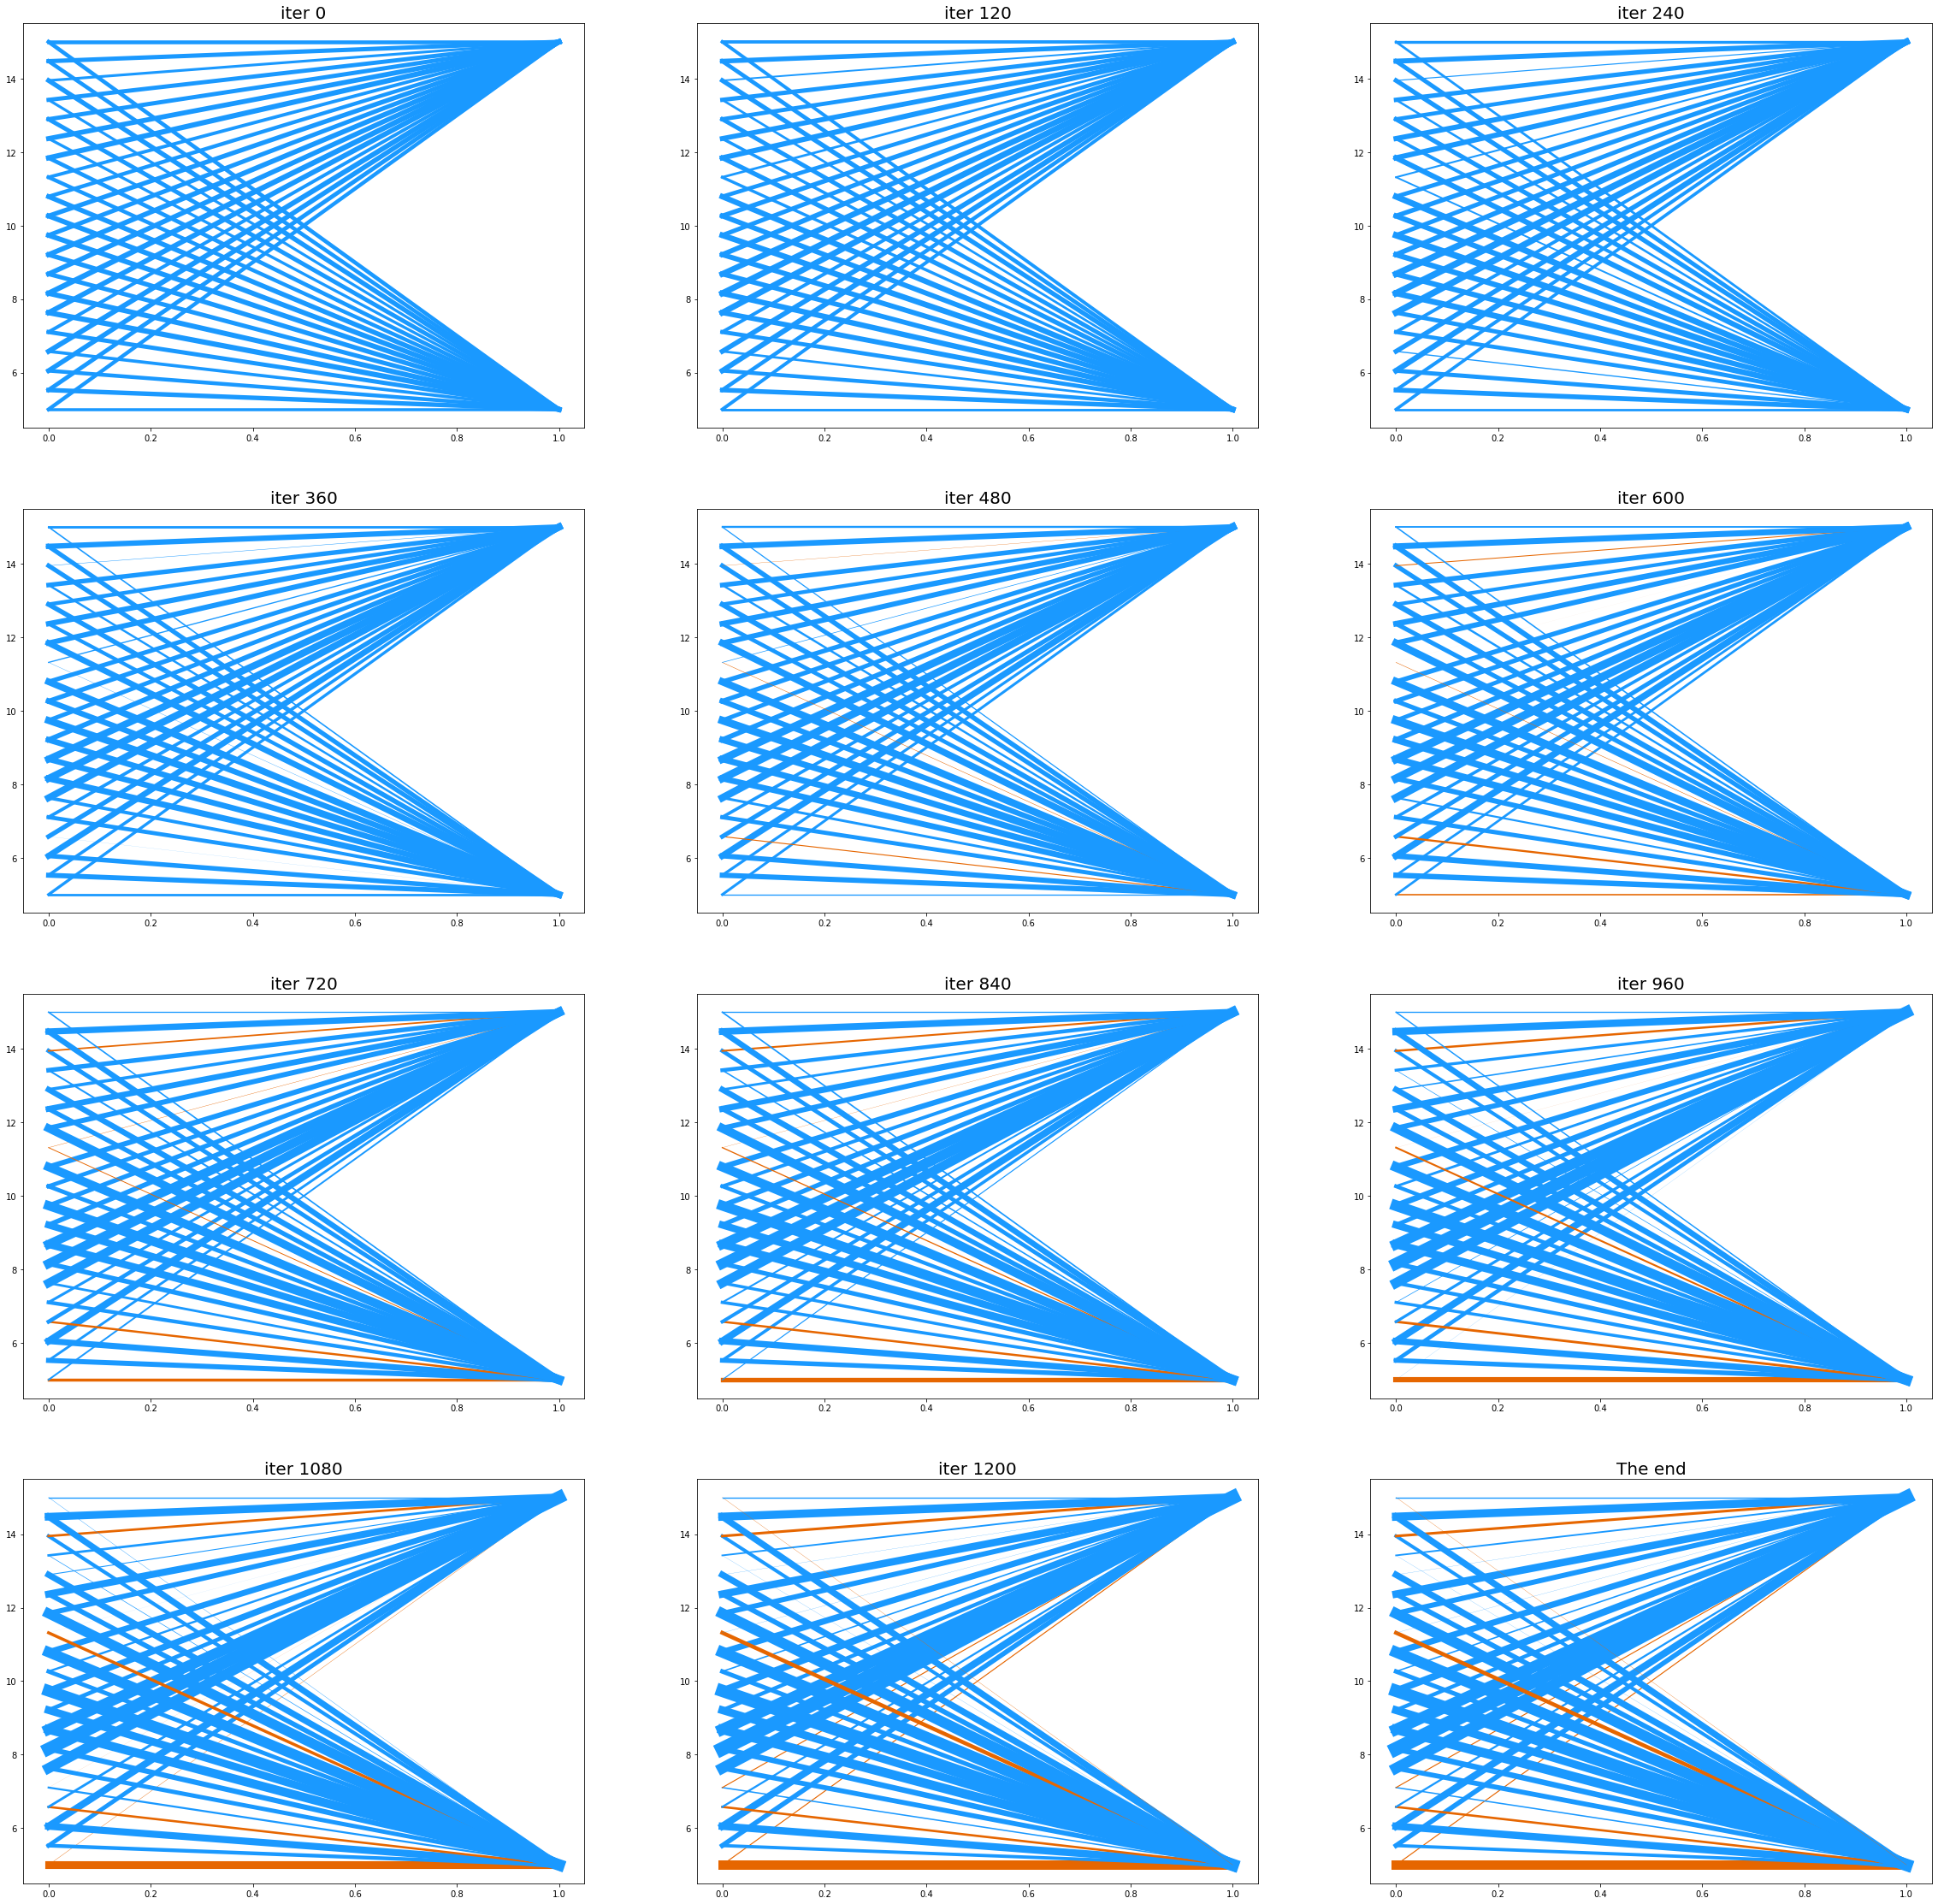
\includegraphics[width=\textwidth]{rstdp_weight1.png}
		\caption{The weight changes when using R-STDP}
		\label{fig:wr1}
	\end{figure}
	
	One of the most successful runs was shown in the figure \ref{fig:wr1}. That model predicted all the 24 samples of the 2 images correctly. The results are demonstrated in the figure \ref{fig:rtest1}. The input weights similarity of the two output neurons was 75\% (shown in the table\ref{table:wr}).
	\begin{table}
		\begin{tabular}{|c|c|c|}
			\hline
			N1 & N2 & diff \\
			-109.85 & -11.72 & -98.13\\
			38.58 & 56.64 & -18.07\\
			85.51 & 81.78 & 3.73\\
			-26.72 & 23.11 & -49.83\\
			15.67 & -11.5 & 27.17\\
			57.1 & 125.98 & -68.88\\
			65.25 & 161.0 & -95.75\\
			108.32 & 132.21 & -23.9\\
			91.74 & 44.37 & 47.36\\
			145.23 & 80.82 & 64.41\\
			51.52 & 16.54 & 34.98\\
			128.9 & 71.96 & 56.95\\
			-46.05 & 1.89 & -47.94\\
			123.59 & 59.73 & 63.86\\
			58.46 & 86.21 & -27.75\\
			74.87 & 1.94 & 72.93\\
			1.87 & 19.16 & -17.29\\
			40.1 & -30.95 & 71.05\\
			74.08 & 95.54 & -21.46\\
			-3.07 & 14.06 & -17.14\\
			\hline
		\end{tabular}
		\hspace{1.5cm}
		\begin{tabular}{|c|c|c|}
			\hline
			N1 & N2 & diff \\
			94.88 & 108.72 & -13.84\\
			81.99 & 38.07 & 43.92\\
			20.26 & 40.82 & -20.56\\
			76.47 & 106.86 & -30.39\\
			42.6 & 143.49 & -100.9\\
			64.68 & 119.8 & -55.11\\
			122.88 & 98.28 & 24.6\\
			55.81 & -43.66 & 99.47\\
			139.63 & 120.11 & 19.52\\
			63.65 & 87.73 & -24.07\\
			120.72 & 9.09 & 111.63\\
			-89.5 & -52.23 & -37.27\\
			70.06 & -5.0 & 75.06\\
			-94.55 & 31.27 & -125.82\\
			60.0 & 96.01 & -36.01\\
			40.33 & -1.31 & 41.64\\
			32.92 & -28.41 & 61.33\\
			-52.81 & 32.44 & -85.25\\
			96.45 & 37.32 & 59.13\\
			46.8 & 88.29 & -41.49\\
			\hline
		\end{tabular}
		\caption{The difference between synaptic weights, after training using the R-STDP. Unlike the STDP method which the weights were 99\% similar, R-STDP depicts larger difference. Here, we show two different training. In the left one (which the weights have been shown in figure \ref{fig:wr1}) the cosine similarity is 75.2\%, and it is 66.4\% for the right one.}
		\label{table:wr}
	\end{table}
	
	\subsection{Test}
	Various executions leads us to distinct results. For instance, there was a 100\% accuracy for 24 tests, which depicted in figure \ref{fig:rtest1}. The weights of this run have been shown in figure\ref{fig:wr1} and in the left table of \ref{table:wr}. This success was mostly thanks to the large contrast between two patterns. Yet, we can see another run where the accuracy was less than 80\%, which shows the huge effect of randomness in R-STDP.
	\begin{figure}[h]
		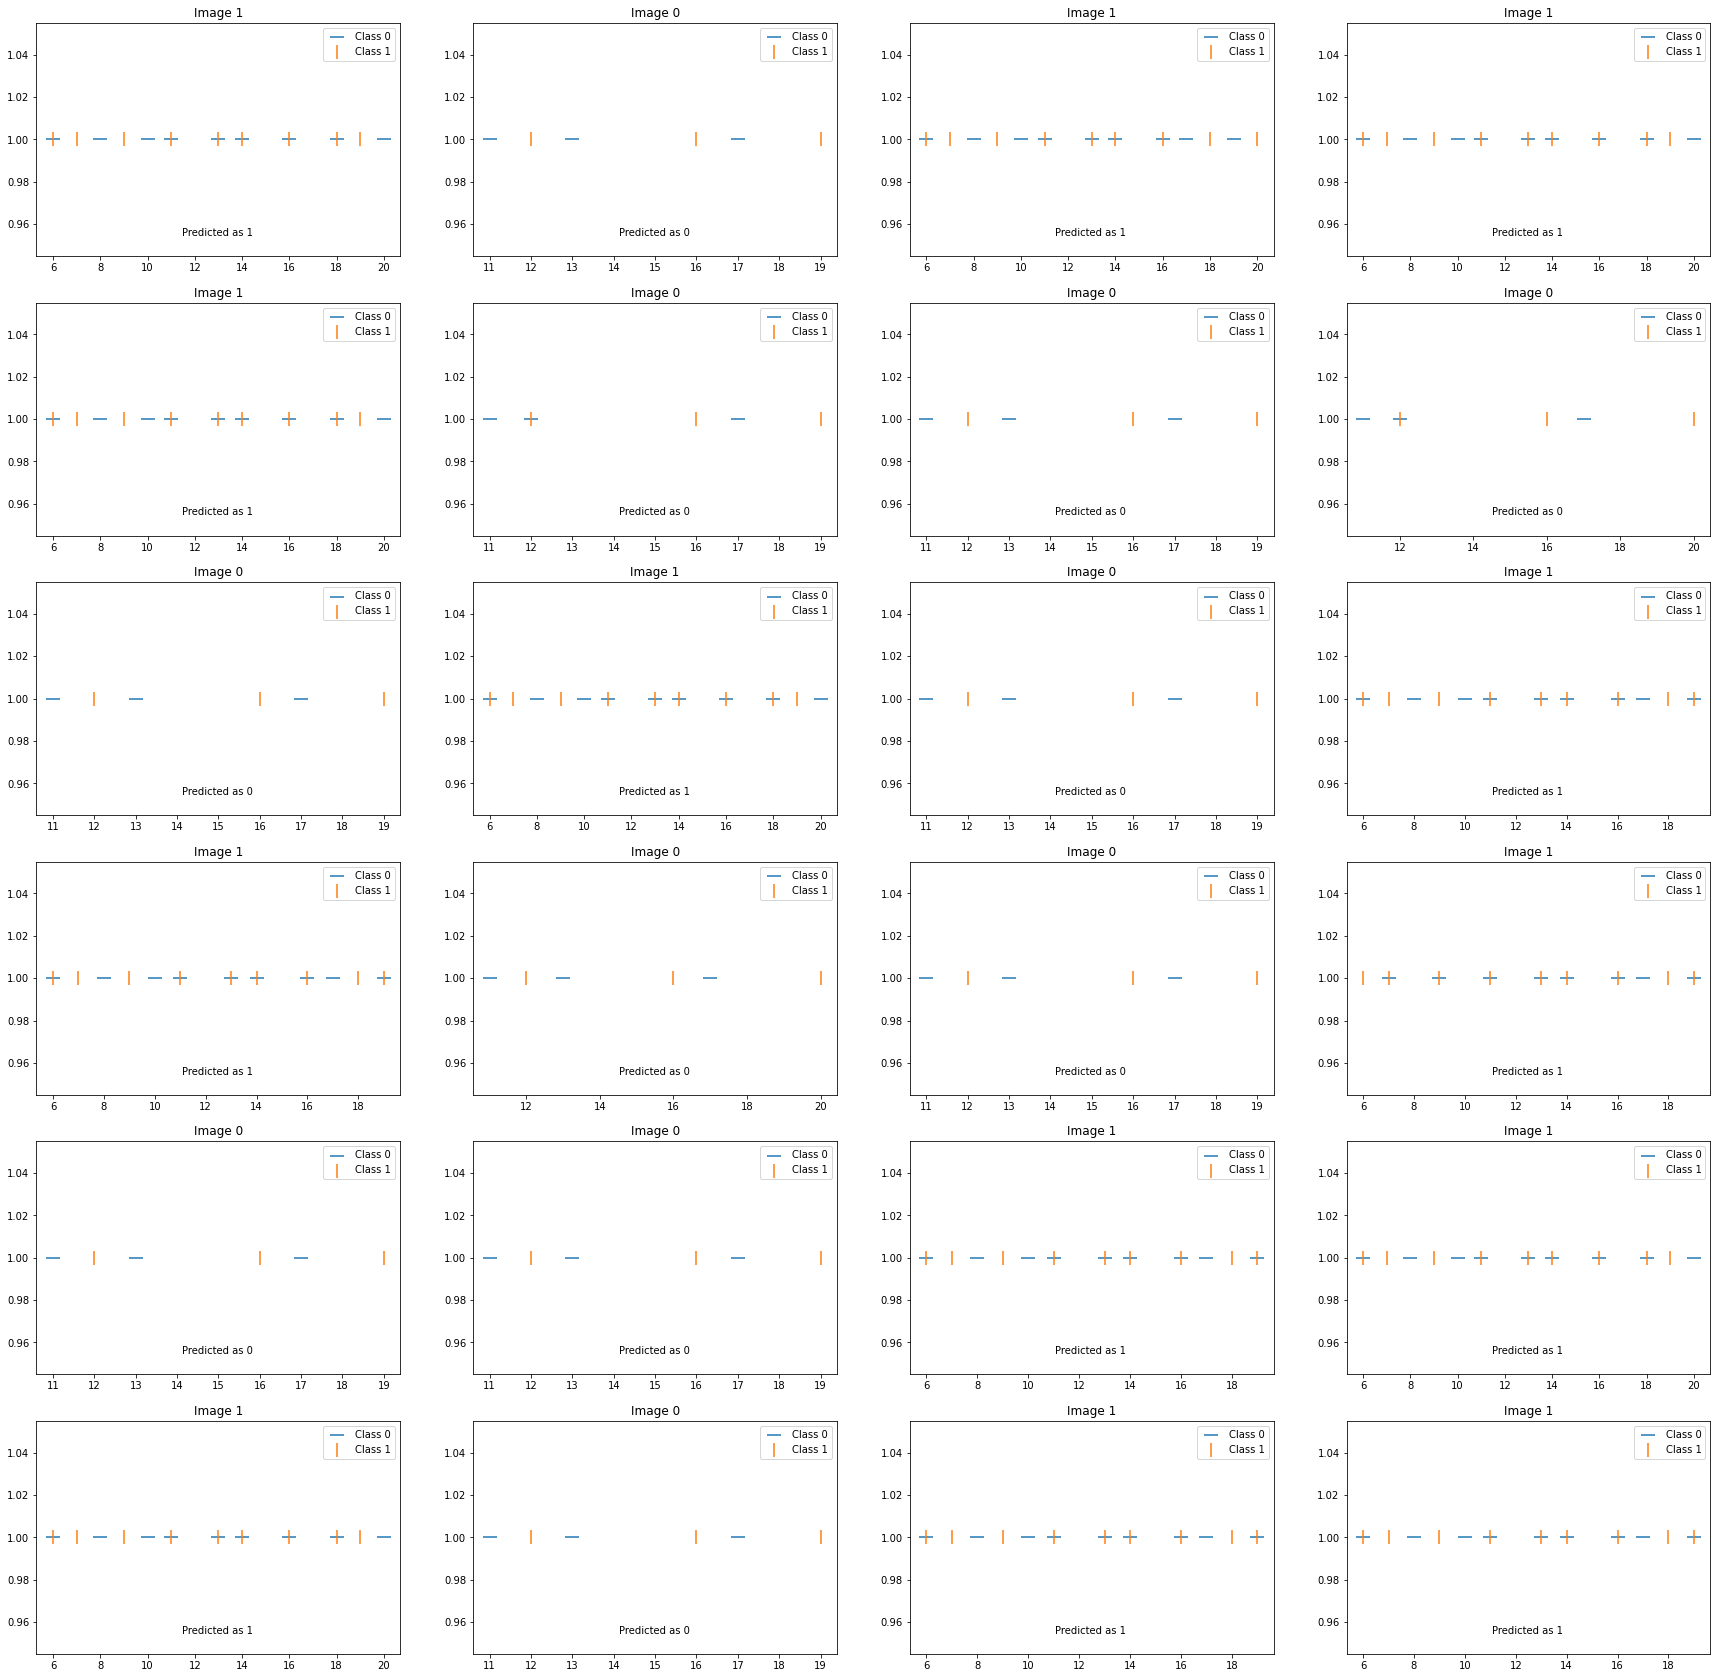
\includegraphics[width=\textwidth]{rstdp_test1.png}
		\caption{The result of one execution of R-STDP learning. Each plot shows the spikes of the two output neurons. The classification has been made upon observing one more spike from an output neuron. In this one, all of the prediction was correct.}
		\label{fig:rtest1}
	\end{figure}
	\begin{figure}[h]
		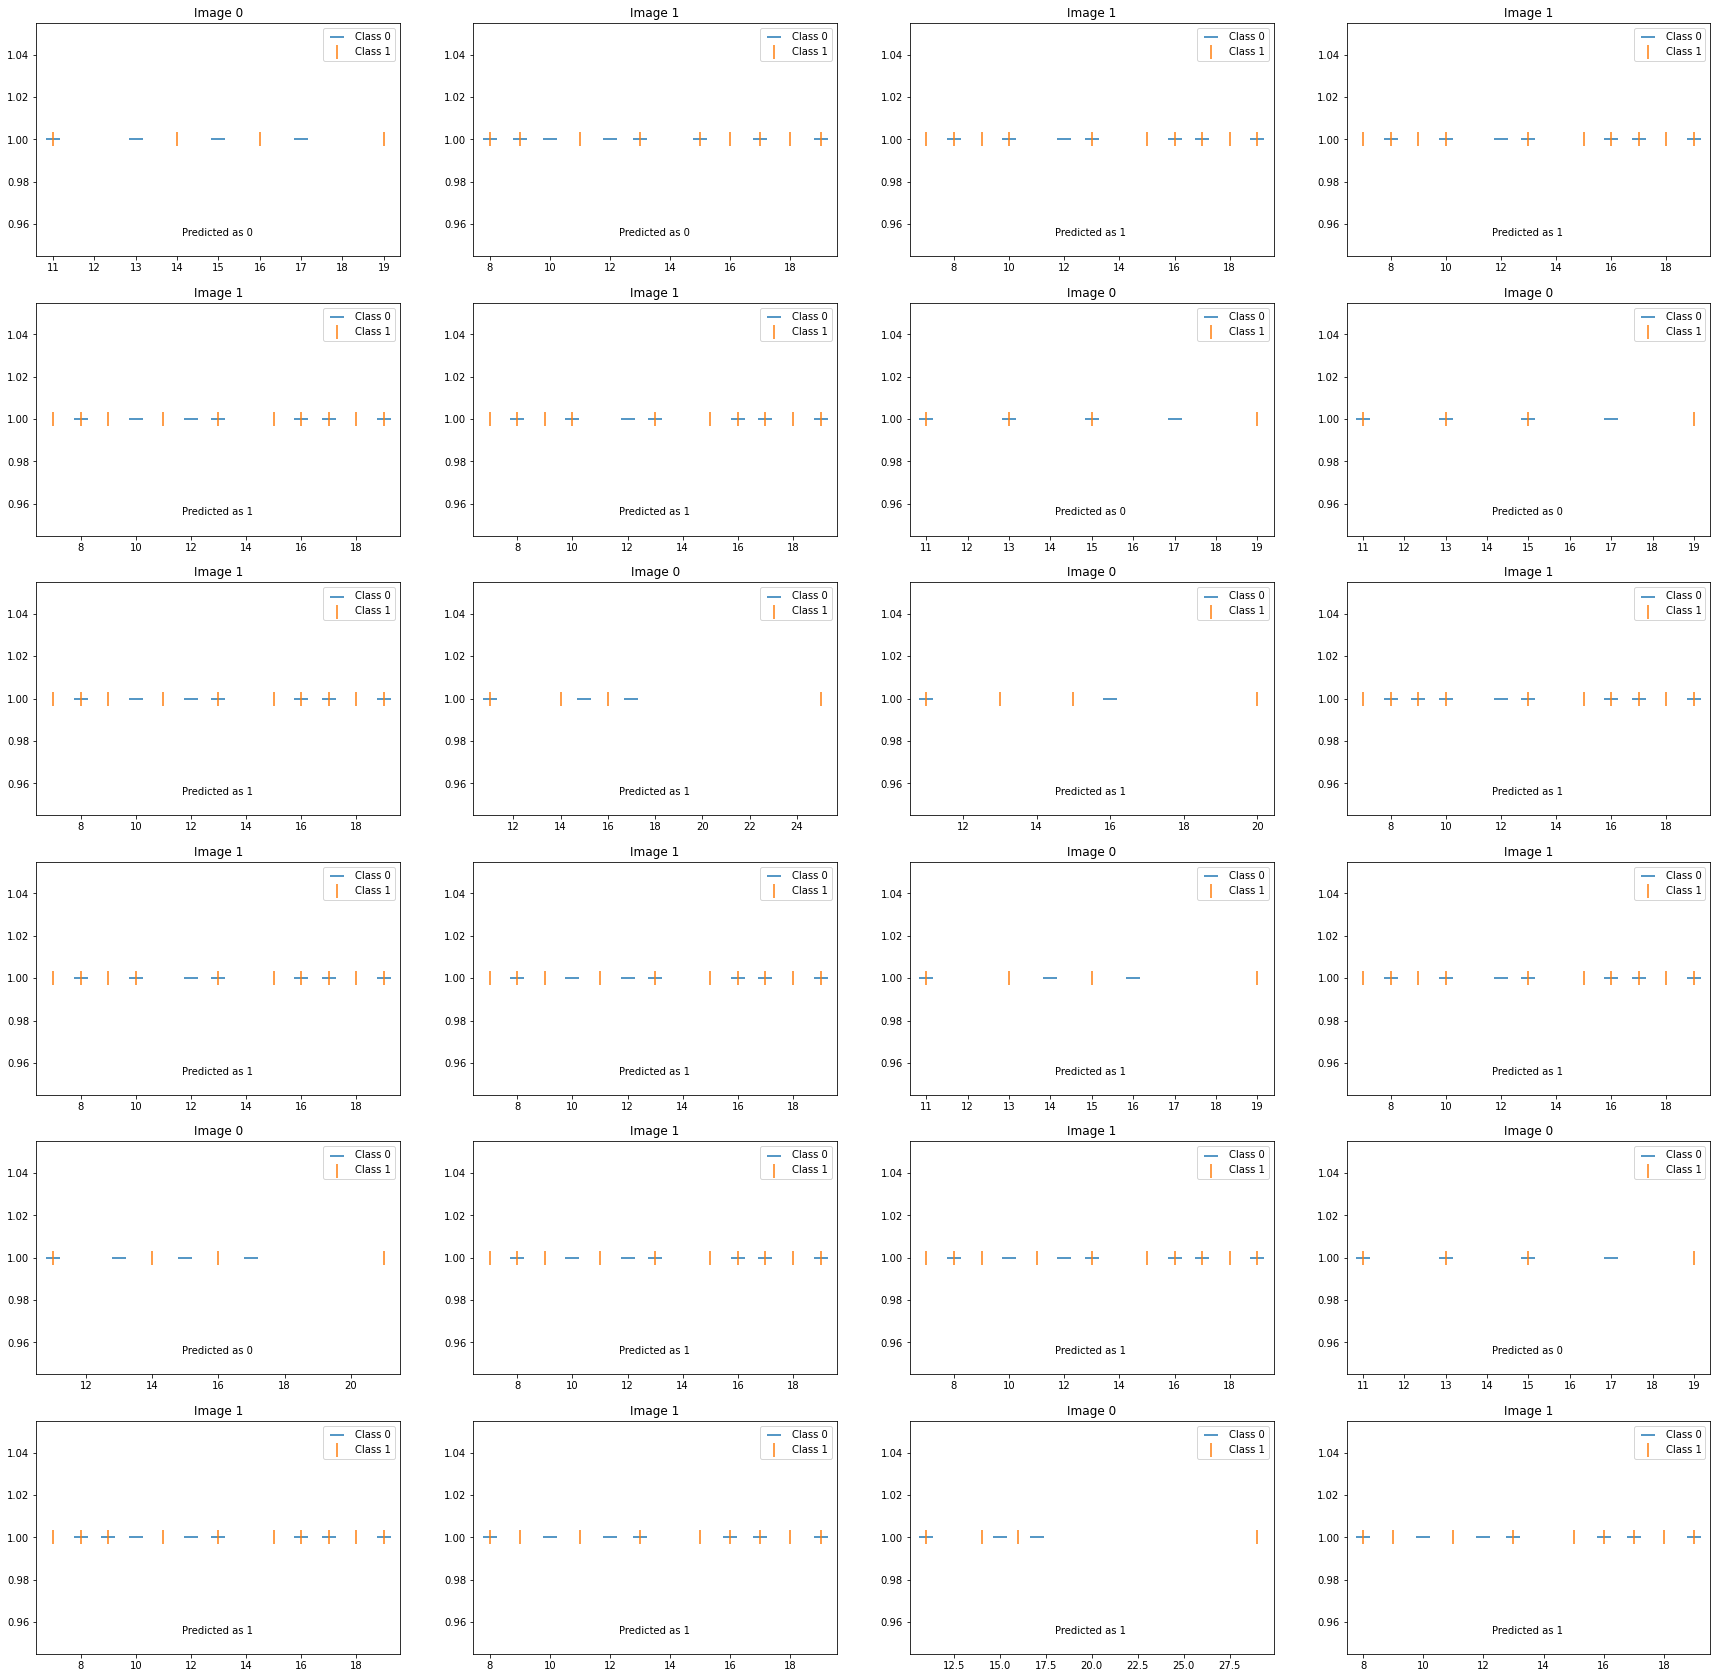
\includegraphics[width=\textwidth]{rstdp_test2.png}
		\caption{The result of another execution of R-STDP learning. Everything was similar to fig\ref{fig:rtest1}, however this time 19 out of the 24 tests was correct (79\% accuracy).}
		\label{fig:rtest2}
	\end{figure}	
	
\end{document}
